% TELOS Governance Trace Architecture
% Standalone compilable TikZ diagram
% Compile with: pdflatex fig4_governance_trace.tex

\documentclass[border=10pt]{standalone}
\usepackage{tikz}
\usetikzlibrary{positioning, arrows.meta, fit, backgrounds}

\begin{document}
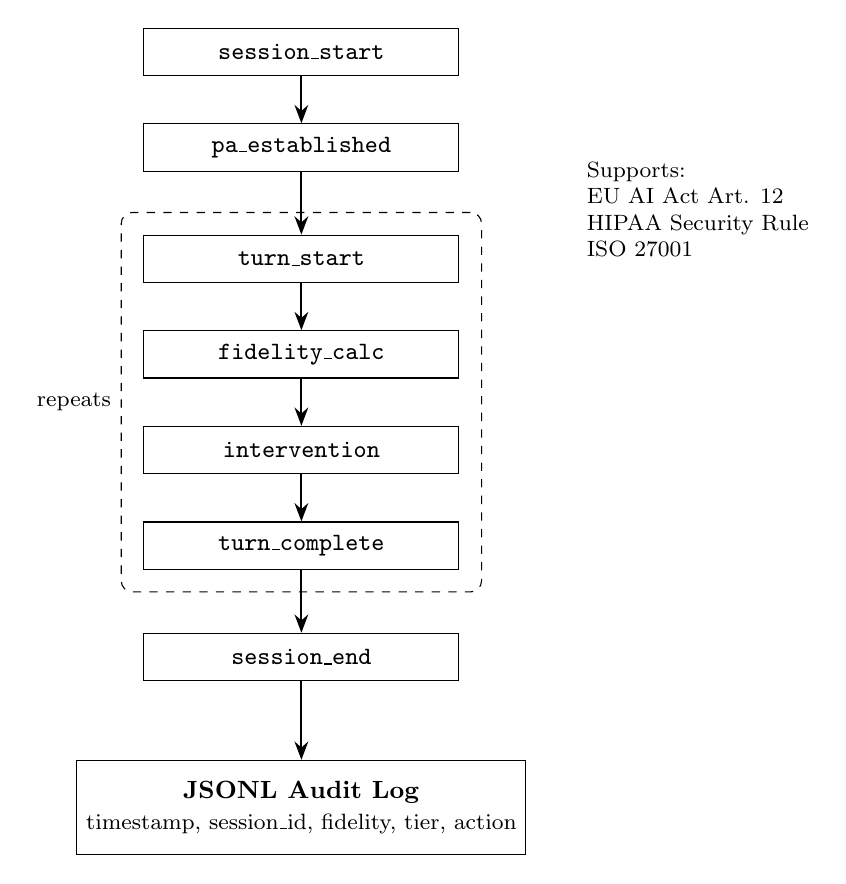
\begin{tikzpicture}[
    >=Stealth,
    node distance=0.6cm,
    event/.style={
        rectangle,
        draw,
        minimum width=4cm,
        minimum height=0.6cm,
        align=center,
        font=\small
    },
    arrow/.style={->, thick}
]

% Session events
\node[event] (start) {\texttt{session\_start}};
\node[event, below=of start] (pa) {\texttt{pa\_established}};

% Turn cycle box
\node[event, below=0.8cm of pa] (turn) {\texttt{turn\_start}};
\node[event, below=of turn] (fid) {\texttt{fidelity\_calc}};
\node[event, below=of fid] (int) {\texttt{intervention}};
\node[event, below=of int] (complete) {\texttt{turn\_complete}};

% Dashed box around turn cycle
\begin{scope}[on background layer]
    \node[draw, dashed, rounded corners, fit=(turn)(fid)(int)(complete), inner sep=8pt, label={[font=\footnotesize]left:repeats}] (cycle) {};
\end{scope}

% Session end
\node[event, below=0.8cm of complete] (end) {\texttt{session\_end}};

% Output
\node[event, below=1cm of end, minimum width=5cm, minimum height=1.2cm] (log) {
    \textbf{JSONL Audit Log}\\
    \footnotesize timestamp, session\_id, fidelity, tier, action
};

% Arrows - simple vertical flow
\draw[arrow] (start) -- (pa);
\draw[arrow] (pa) -- (turn);
\draw[arrow] (turn) -- (fid);
\draw[arrow] (fid) -- (int);
\draw[arrow] (int) -- (complete);
\draw[arrow] (complete) -- (end);
\draw[arrow] (end) -- (log);

% Compliance note
\node[font=\footnotesize, anchor=west, align=left] at (3.5, -2) {
    Supports:\\
    EU AI Act Art. 12\\
    HIPAA Security Rule\\
    ISO 27001
};

\end{tikzpicture}
\end{document}
